%
\section{Practical foundations}
\label{sec_3}

After the formal and logical foundations this chapter introduces
the practical aspects of building and using such a logic to build
reliable distributed systems is presented. This section covers Raft,
a state of the art protocol to build distributed systems.
Afterwards, a way to additionally harden such systems by using
the \textit{proofs-as-programs} approach is described.
This includes a short explenation of \textit{COQ} as well as
\textit{Velisarios} which is used to implement the \textit{RAFT}
consensus protocol.

\subsection{Consensus Algorithms}
As mentioned in the introduction, distributed systems are useful to harden
critical infrastructures. A critical infrastructure is one where failures
of single components could lead to a desaster. So the informations and
actions of single components shall be distributed and replicated to multiple
components holding the same state. The distributed system manages a
global state which is replicated over multiple members of the system and
a failure of some members can be tolerated. To harden the system further
the definition of failure is slightly different.~\cite{rahli2018velisarios}

\begin{defi}
  A byzantine failure is a failure which imposes no conditions.
\end{defi}

This means that a failure could happen at any time and the distributed
system has no relaible way to detect that a member failed or is malfunctioning.
Furthermore, a member could distribute false informations across the network
and the system has to react reliable consistent to a certain limit a failures.~\cite{lamport1982byzantine}

\begin{defi}
  A typical byzantine fault-tolerant system can tolerate $n=3f+1$ failures
  where $n$ gives the amount of members in the network to tolerate $f$ byzantine
  members.
\end{defi}

\begin{defi}
  A consensus protocol is an algorithm that allows a network of machines to
  agree on a common state of the network. The members act as a coherent
  group which could tolerate failures of individual members.
\end{defi}

A consensus protocol is a state-of-the-art approach to build reliable and
resilent distributed systems which can tolerate byzantine failures.

\begin{figure}[ht]
  \centering
  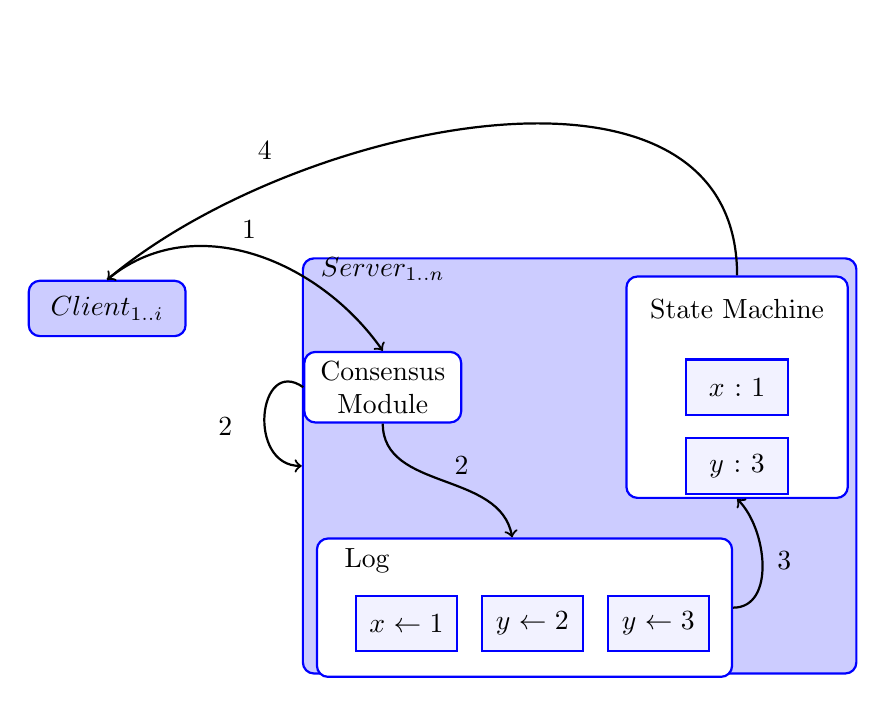
\begin{tikzpicture}[
    auto,
    block/.style={
      rectangle,
      draw=blue,
      thick,
      fill=blue!20,
      text width=5em,
      align=center,
      rounded corners,
      minimum height=2em
    }]

    % client box
    \draw (-6,2) node[block] (C) {$Client_{1..i}$};
    % server box
    \draw (0,0) node[
    block,
    minimum height=15em,
    minimum width=20em] (N) {};
    \node at (-2.5,2.5) {$Server_{1..n}$};
    % consensus
    \draw (-2.5,1) node[block,fill=white] (M) {Consensus Module};
    % log
    \draw (-0.7,-1.8) node[
    block,
    fill=white,
    minimum width=15em,
    minimum height=5em] (L) {};
    \node at (-2.7,-1.2) {Log};
    \draw (-2.2,-2) node[block,fill=blue!5,sharp corners,text width=3em] {$x\leftarrow 1$};
    \draw (-0.6,-2) node[block,fill=blue!5,sharp corners,text width=3em] {$y\leftarrow 2$};
    \draw (1,-2) node[block,fill=blue!5,sharp corners,text width=3em] {$y\leftarrow 3$};

    % state machine
    \draw (2,1) node[
    block,
    fill=white,
    minimum height=8em,
    minimum width=8em] (S) {};
    \node at (2,2) {State Machine};
    \draw (2,1) node[block,fill=blue!5,sharp corners,text width=3em] {$x: 1$};
    \draw (2,0) node[block,fill=blue!5,sharp corners,text width=3em] {$y: 3$};

    % lines
    \draw[->, thick] (C.north) to[out=40,in=125] (M.north) node at (-4.2,3) {1};
    \draw[->, thick] (M.south) to[out=-90,in=100] (L) node at (-1.5,0) {2};
    \draw[->, thick] (M.west) to[out=145,in=180,distance=2em] (N.west) node at (-4.5,0.5) {2};
    \draw[->, thick] (L.east) to[out=0,in=-45] (S.south) node at (2.6,-1.2) {3};
    \draw[->, thick] (S.north) to[out=90,in=40] (C.north) node at (-4,4) {4};
  \end{tikzpicture}
  \caption{Overview of the replicated state machine architecture.~\cite{ongaro2014search}}
  \label{fig:pbftsm}
\end{figure}

In figure~\ref{fig:pbftsm} an overview of the generic structures of the
replicated state machine architecture is presented. Most protocols using
replicated state machines act in the same manner. A possible bunch of clients
send their requests to the distributed network (1). The network can consist
of multiple servers. The consensus module is the middleware implementation of
the consensus protocol and acts as mediator between the clients and servers.
The request is forwarded to all server consensus modules within the network (2).
Also the request is added to the server log. The request is seen as a command to
the server state machine and gets applied if the majority of the network
recieved the new command (3). Afterwards, the client recieves the result (4).
All server logs contain the same commands in the same order. So the servers
state machines process the commands in the same order and produce the same output.~\cite{ongaro2014search}

The major parts of the consensus algorithm are to ensure that the logs are
consistent across the servers, to manage the client network communication,
handle the replication across the network and keep the network alive if
some server fails. So a consensus algorithm ensures the following properties:~\cite{ongaro2014search}

\begin{itemize}
\item Ensure safty under all non-Byzantine conditions.
\item Ensure availability as long as the majority of servers is
  functional and can communicate.
\item Consistency doesn't depend on timing.
\item The system performance depends on the majority of servers
  and minarities can be ignored.
\end{itemize}

One early approach to build such distributed systems was presented by
Leslie Lamport et al as Paxos in~\cite{lamport1978time}.
Most of the newer protocols are directly derived from the early Paxos
protocol like~\cite{lamport2001paxos, van2015paxos}.
As Ongaro et al stated in~\cite{ongaro2014search} the family of
Paxos protocols suffer from two problems. Besides they ensure the
properties and provide a efficent protocol, the protocols are
difficult to understand. The descriptions are ``notoriously
opaque''~\cite{ongaro2014search} and are mostly focused on a
subset of the real world protocol. The other problem is that the
most descriptions are not implementation ready and a huge effort
is needed to complete the missing parts of the protocol.
So, real implementation reflect the paxos protocol only at
the beginning. To tackle these problems Ongaro et al made
the effort to design a new consensus protocol without the
Paxos history. This new protocol RAFT was designed with
understandability in mind. This means, that the implementers
effort needs to be minimized and the description and pseudo-code
needs to be as close to the real world as possible. Also,
the properties mentioned before needs to be taken into account.
The resulting protocol shall be efficient and safe under
typical conditions and operations.~\cite{ongaro2014search}



\subsubsection*{The RAFT protocol}
The algorithm is designed to manage a replicated log
across a distributed network. The protocol uses a leader-based
approach where one distinguished leader takes the full responsibility
for log replication and client handling. The other nodes are
only serving as replicas without own intentions. This approach
leads to a three main components which can be viewed quite separated.~\cite{ongaro2014search}

\begin{itemize}
\item Leader election: Elect a new leader if the existing leader fails.
\item Log replication: The leader manages client requests and takes care
  of replicating his log across the network.
\item Safety:  The key property is the state machine safety which means that
  if any server has applied a log entry no other server applies a
  different log entry at the same log index.
\end{itemize}

The last point is a set of five properties to ensure the liveness and
safety of the Raft protocol. The individual points are discussed at
their belongings.~\cite{ongaro2014search}

\begin{itemize}
\item Election safety: At all times at most one leader can be elected.
\item Leader Append-Only: New entries are only appended to the log and
  a leader never overwrites or deletes entries from it's log.
\item Log Matching: If an entry is contained in two logs with the same
  term and index, these logs are identical up til the entries index.
\item Leader Completness: If an entry is committed in some term, then the
  entry is present in all leader logs in all higher terms.
\item State Machine Safety: If an log entry with some index is applied to
  the internal state machine, then no other server ever applies a
  different log entry at the same index.
\end{itemize}

\paragraph{Basics}
A consensus protocol doesn't use real time to measure the protocol progress
instead the time is divided into abstracts chunks of time. These chunks
serve as the logical clock of the protocol.~\cite{ongaro2014search}

\begin{defi}
  Time is divided into terms of arbitrary length where each term
  starts with an election phase which can be followed by a normal
  operation phase.
\end{defi}

This can be seen in figure~\ref{fig:terms}. The first term starts with an
election phase followed by a normal operation phase. The leader fails and
the term ends. The next terms starts with an election phase which results in no
new leader and the next term is started.
Terms are numbered by consecutive integers and servers may observe term
transitions at different times. Each server stores it current term number
and exchanges it at every communication to detect failed leaders or outdated
data.~\cite{ongaro2014search}

\begin{figure}[ht]
  \centering
  \begin{tikzpicture}[>=stealth',shorten >=1pt,auto,node distance=4cm,semithick]

    \draw[->] (-5,0) -- (5,0) node at (5,-0.5) {terms};
    % first term
    \draw (-4,0.5) -- (-4,-0.5);
    \draw (-3,0.5) -- (-3,-0.5);
    \draw (-1.5,0.5) -- (-1.5,-0.5);
    \draw[decoration={brace,mirror,raise=5pt},decorate] (-4,-0.5) -- node[below=12pt] {$term_1$} (-1.5,-0.5);
    \draw[decoration={brace,raise=5pt},decorate] (-4,0.5) -- node[above=8pt] {\scriptsize$election$} (-3,0.5);
    \draw[decoration={brace,raise=5pt},decorate] (-3,0.5) -- node[above=15pt] {\scriptsize$normal\ operation$} (-1.5,0.5);


    % second term
    \draw (-0.5,0.5) -- (-0.5,-0.5);
    \draw (0.5,0.5) -- (0.5,-0.5);
    \draw[decoration={brace,mirror,raise=5pt},decorate] (-0.5,-0.5) -- node[below=12pt] {$term_2$} (0.5,-0.5);
    \draw[decoration={brace,raise=5pt},decorate] (-0.5,0.5) -- node[above=8pt] {\scriptsize$split\ vote$} (0.5,0.5);

    %third term
    \draw (4,0.5) -- (4,-0.5);
    \draw (2,0.5) -- (2,-0.5);
    \draw (1.5,0.5) -- (1.5,-0.5);
    \draw[decoration={brace,mirror,raise=5pt},decorate] (1.5,-0.5) -- node[below=12pt] {$term_3$} (4,-0.5);
    \draw[decoration={brace,raise=5pt},decorate] (1.5,0.5) -- node[above=8pt] {\scriptsize$election$} (2,0.5);
    \draw[decoration={brace,raise=5pt},decorate] (2,0.5) -- node[above=15pt] {\scriptsize$normal\ operation$} (4,0.5);

  \end{tikzpicture}
  \caption{Example timeline within the protocol process.}
  \label{fig:terms}
\end{figure}

A server can be in one of three possible states at all times.
A server can either be a \textit{leader}, a \textit{follower} or a
\textit{candidate}. Figure~\ref{fig:serverstates} shows the state
and the transition between them. Only one leader is allowed in normal operation
and all other servers are passive followers which obey the leaders commands.
The followers aren't issueing requests on their own (except message forwardng to
the current leader) and only respond to requests from the leader and candidates.
The leader handles all client communication and manages log replication across
the followers. The candidate state is only entered if the leader fails and
a new leader needs to be elected.~\cite{ongaro2014search}

\begin{figure}[ht]
  \centering
  \begin{tikzpicture}[->,>=stealth',shorten >=1pt,auto,node distance=4cm,
    semithick]
    \tikzstyle{every state}=[rectangle]

    \node[initial,state] (A) {$Follower$};
    \node[state]         (B) [right of=A] {$Candidate$};
    \node[state]         (C) [right of=B] {$Leader$};

    \draw (A.north) to[out=45,in=125] (B.north west) node[align=left] at (0,1.5) {times out\\start election};
    \draw (B.north) to[out=125,in=45,distance=5em] (B.north) node[align=left] at (4,2) {times out\\new election};
    \draw (B.north east) to[out=45,in=125] (C.north) node[align=left] at (8,1.5) {recieves votes from majority};
    \draw (B.south) to[out=-125,in=-45] (A.south east) node[align=left] at (4,-3) {discovers server with higher term};
    \draw (C.south) to[out=-125,in=-45] (A.south) node[align=left] at (5,-1.5) {discovers current leader\\or new term};

  \end{tikzpicture}
  \caption{The server state transistions diagram.~\cite{ongaro2014search}}
  \label{fig:serverstates}
\end{figure}

\paragraph{Leader election}
As stated in the figure~\ref{fig:serverstates} raft uses timeouts to handle
leadership and election. Thus, every server has an internal timer with a
random time (mostly between 150 and 300ms) which gets resetted with
every message from a leader. Besides normal messages the leader uses
heartbeat messages to reset the follower timers if the cluster is idle.
If a follower recieves no messages over a period of time the
follower gets an \textit{election timeout}. It assumes the leader
failed and turns into candidate state starting a new term and
election. The election runs as follows:~\cite{ongaro2014search}

\begin{enumerate}
\item A follower times out by recieving no messages over a period of time.
\item A follower increments its current term and turns into candidate state.
\item A candidate votes for itself and issues the vote to the cluster.
\item Continue with point one until one of the follwing happens:
  \begin{enumerate}
  \item The candidate wins the election.
  \item Another candidate wins the election.
  \item The election times out with no winner.
  \end{enumerate}
\end{enumerate}

Since this maybe happens in parallel on many servers more details
need to take into account when determing the possible outcomes.

(a) A candidate wins the election when it recieves the majority of
votes in the cluster. Each server votes for one candidate on a
\textit{first-comes-first-served} basis. The majority voting ensures
the only one leader safety property. The winner imediatly starts
by sending heartbeat messages to all other servers to implement itself
as new leader and stop the election phase.~\cite{ongaro2014consensus}\\
(b) A candidat may recieve messages from a possible new leader.
The new leader is accepted if it's term is at least as large as
the candidates one. The candidate accepts the new leader and turns
into follower state. Otherwise, the leader is rejected and the election
goes on.~\cite{ongaro2014consensus}\\
(c) If multiple candidates start with the election at the same
time or the network connection is poor enough no candidate may win
the election. In this split vote scenario the candidate times out again
and starts a new term and election phase.\cite{ongaro2014consensus}

\paragraph{Log replication}

\begin{figure}[ht]
  \centering
  \begin{tikzpicture}[>=stealth',shorten >=1pt,auto,node distance=4cm,semithick]

    \draw[->] (-5,0) -- (3.9,0) node at (0,-0.5) {committed entries};
    \draw[-] (-5,0.2) -- (-5,-0.2);

    % first log
    \node at (-4.4,1) [draw,thick,rectangle,align=center,minimum height=1.2cm] {$1$\\$x\leftarrow 3$};
    \node at (-3.15,1) [draw,thick,rectangle,align=center,minimum height=1.2cm] {$1$\\$y\leftarrow 1$};
    \node at (-1.9,1) [draw,thick,rectangle,align=center,minimum height=1.2cm] {$1$\\$y\leftarrow 9$};
    \node at (-0.65,1) [draw,thick,rectangle,align=center,minimum height=1.2cm] {$2$\\$x\leftarrow 2$};
    \node at (0.61,1) [draw,thick,rectangle,align=center,minimum height=1.2cm] {$3$\\$x\leftarrow 0$};
    \node at (1.87,1) [draw,thick,rectangle,align=center,minimum height=1.2cm] {$3$\\$y\leftarrow 7$};
    \node at (3.13,1) [draw,thick,rectangle,align=center,minimum height=1.2cm] {$3$\\$x\leftarrow 5$};
    % second log
    \node at (-4.4,2.5) [draw,thick,rectangle,align=center,minimum height=1.2cm] {$1$\\$x\leftarrow 3$};
    \node at (-3.15,2.5) [draw,thick,rectangle,align=center,minimum height=1.2cm] {$1$\\$y\leftarrow 1$};
    % third log
    \node at (-4.4,4) [draw,thick,rectangle,align=center,minimum height=1.2cm] {$1$\\$x\leftarrow 3$};
    \node at (-3.15,4) [draw,thick,rectangle,align=center,minimum height=1.2cm] {$1$\\$y\leftarrow 1$};
    \node at (-1.9,4) [draw,thick,rectangle,align=center,minimum height=1.2cm] {$1$\\$y\leftarrow 9$};
    \node at (-0.65,4) [draw,thick,rectangle,align=center,minimum height=1.2cm] {$2$\\$x\leftarrow 2$};
    \node at (0.61,4) [draw,thick,rectangle,align=center,minimum height=1.2cm] {$3$\\$x\leftarrow 0$};
    \node at (1.87,4) [draw,thick,rectangle,align=center,minimum height=1.2cm] {$3$\\$y\leftarrow 7$};
    \node at (3.13,4) [draw,thick,rectangle,align=center,minimum height=1.2cm] {$3$\\$x\leftarrow 5$};
    \node at (4.4,4) [draw,thick,rectangle,align=center,minimum height=1.2cm] {$3$\\$x\leftarrow 4$};
    % fourth log
    \node at (-4.4,5.5) [draw,thick,rectangle,align=center,minimum height=1.2cm] {$1$\\$x\leftarrow 3$};
    \node at (-3.15,5.5) [draw,thick,rectangle,align=center,minimum height=1.2cm] {$1$\\$y\leftarrow 1$};
    \node at (-1.9,5.5) [draw,thick,rectangle,align=center,minimum height=1.2cm] {$1$\\$y\leftarrow 9$};
    \node at (-0.65,5.5) [draw,thick,rectangle,align=center,minimum height=1.2cm] {$2$\\$x\leftarrow 2$};
    \node at (0.61,5.5) [draw,thick,rectangle,align=center,minimum height=1.2cm] {$3$\\$x\leftarrow 0$};
    % fifth log
    \node at (-4.4,7) [draw,thick,rectangle,align=center,minimum height=1.2cm] {$1$\\$x\leftarrow 3$};
    \node at (-3.15,7) [draw,thick,rectangle,align=center,minimum height=1.2cm] {$1$\\$y\leftarrow 1$};
    \node at (-1.9,7) [draw,thick,rectangle,align=center,minimum height=1.2cm] {$1$\\$y\leftarrow 9$};
    \node at (-0.65,7) [draw,thick,rectangle,align=center,minimum height=1.2cm] {$2$\\$x\leftarrow 2$};
    \node at (0.61,7) [draw,thick,rectangle,align=center,minimum height=1.2cm] {$3$\\$x\leftarrow 0$};
    \node at (1.87,7) [draw,thick,rectangle,align=center,minimum height=1.2cm] {$3$\\$y\leftarrow 7$};
    \node at (3.13,7) [draw,thick,rectangle,align=center,minimum height=1.2cm] {$3$\\$x\leftarrow 5$};
    \node at (4.4,7) [draw,thick,rectangle,align=center,minimum height=1.2cm] {$3$\\$x\leftarrow 4$};
    
    \draw[decoration={brace,mirror,raise=5pt},decorate] (5,0.3) -- node[right=15pt] {followers} (5,6);
    \node at (5,7) [right=15pt] {leader};
    \node at (5,8.5) [right=15pt] {log index};
    \node at (-4.4,8.5) {1};
    \node at (-3.15,8.5) {2};
    \node at (-1.9,8.5) {3};
    \node at (-0.65,8.5) {4};
    \node at (0.61,8.5) {5};
    \node at (1.87,8.5) {6};
    \node at (3.13,8.5) {7};
    \node at (4.4,8.5) {8};
    
  \end{tikzpicture}
  \caption{An example of logs and it's entries accross a cluster.~\cite{ongaro2014consensus}}
  \label{fig:logs}
\end{figure}


%One early approach to build distributed systems based on consensus
% is the family of Paxos protocols first introduced by Leslie Lamport
% et al in~\cite{lamport1978time} and adjusted by many others,
% like~\cite{lamport2001paxos, van2015paxos}. As mentioned by
% Ongario et al in~\cite{ongaro2014search} the Paxos protocols
% are quite difficult to understand.



% Distributed systems are very useful to harden critical infrastructures.
% Imagine a nuclear powerplant where every failure in the controlling computer
% system could led to a catastroph. Such important system should be relicated
% among a different computer located at different locations. These distributed
% system manges a commen state among all participants. This can be done by
% using \textit{consensus protocols} and state machines to manage a global state among
% the network. Such protocols allow machines to act as a coherent group which
% can tolerate failures of individual machines.~\cite{rahli2018velisarios, ongaro2014search}


\subsection{COQ}
COQ is an interactive proof assistant which enables users to formalize
specifications and develop programs that fullfill these pecifications.
These tools are developed for domains that require high standards in
development and verification of programs. Also, it enables computer
scientist and mathematicians to develop proofs in an expressive
higher-order logic.~\cite{the_coq_development_team_2019_2554024}
The formalism used to provide such features is the \textit{Calculus of Inductive
  Construction}. It's a language that aims to represent functional programs
in a ML language style and proofs in higher order logic (HOL).
It uses inductive definitions to represent data-structures, even infinite
ones. Based on the Curry-Howard-Isomorphism, COQ uses an approach based
on the \textit{Calculus of Construction} as logical
background or metalanguage as described in the proofs-as-programs sections.~\cite{the_coq_development_team_2019_2554024, paulinmohring:hal-01094195}

The Calculus of Construction is a typed polymorphic language which can
represent inductive definitions. It is the underlying language for the
Calculus of Inductive Construction. It is a pure and riched typed $\lambda$
lambda-calculus which can describe terms and types.~\cite{paulinmohring:hal-01094195}
The term includes the normal lambda operations, like binding, abstraction
and application. The typing supports for instance  abstractions with
dependent products and typing of types. These typing allows to ``sort''
(a special COQ constant) types in universes and apply to them differently
depending on the certain universe of objects.~\cite{paulinmohring:hal-01094195}


Inductive definitions are build on top of the pure type system.
\begin{defi}
  An inductive definitions consists of a name, a type (defined by the arity)
  and a set of constructors, for instance \texttt{Inductive N : Type := O : N |
    S : N $\rightarrow$ N}.
\end{defi}


% Proof assistents are designed to support developers to proof mathematical
% statements, write formal specifications and verify the correctness of programs.
% One of these systems is COQ which uses the specification language
% \textit{Gallina}. Gallina can represent programs, properties of programs
% and proofs of these properties. Through the already mentioned
% Curry-Howord-Isomorphism the specifications are represented by
% \textit{Calculus of Inductive Construction}. This is a rich typed $\lambda$ calculus and
% can be extracted to either \textit{Ocaml} or \textit{Haskell}.~\cite{the_coq_development_team_2019_2554024}

% \paragraph{Gallina}
% As already mentioned in the proof-as-programs paragraph, the metalanguage to
% describe mathematical theories and prove the specifications of programs.
% A theorie can consists out of numerous axioms, hypothesis, parameters,
% lemmas, theorems and definitions for sets, predicates, functions and constants.
% These are the logical objects describing a theorie.
% The objects are described as terms which are typed. Types are described
% using the same syntax as term and is a semantically subclass of term.~\cite{the_coq_development_team_2019_2554024}
% The full syntax description can be found in the reference manual~\cite{the_coq_development_team_2019_2554024}.

% \paragraph{Calculus of Inductive Construction}
% The underlying formal language of COQ is the Calculus of Inductive Construction
% (Cic). Every expression or term in COQ have a type and Cic is the inference
% system that checks the types of logical objects for correctness.
% Every object that is handled by the formalism has some form of type whether it
% be a basic datatype or more complex variants.~\cite{the_coq_development_team_2019_2554024}

% \begin{defi}
%   In COQ a type is represented by $x:T$ which could be read as the element $x$
%   that belongs to the type $T$. Types of types are named sorts which belong to
%   the possible infinite but well-founded typing hierarchy or algebraic universe.
% \end{defi}

\paragraph{Extraction}
COQ offers the possibillity to extract typed checked logical objects into
other programming languages. In this thesis the resulting code is extracted
as Ocaml library which can be used to run and simulate the implemented
protocol.



\subsection{Velisarios}
The Logic of Events as presented in the last chapter is able to
handle inconsistent distributed networks. Distributed systsms which are
able to tolerate a specific amount of failed nodes or imperfect
information about the network state share the common property of
byzantine fault-tolerance. This is named after the \textit{Byzantine Generals
  Problem} described by Leslie Lamport in~\cite{}.





Rahli et al presented an implementation of the logic of event
in~\cite{rahli2018velisarios}. The implementation is written
for the COQ theorem prover in the internal specification language,
the calculus of construction. The framework supports to develop
\textit{byzantine fault-tolerant} protocols in the implementation
and mechnical proofing.~\cite{rahli2018velisarios}

% \begin{defi}
%   A byzantine fault-tolerant state-machine replication (BFT-SMR) is
%   a state of the art technique to harden distributed systems.
% \end{defi}


%%% Local Variables:
%%% mode: latex
%%% TeX-master: "../master"
%%% End:
